% CHAPTER 3
\chapter{Proposed Methodology}

\section{System Overview}

The architecture of SARAS (Search And Rescue Autonomous Swarm) is formulated as an end-to-end, multi-tier robotic and artificial intelligence framework designed to overcome the vulnerabilities of single-operator and centralized aerial search platforms. The core operational loop connects physical sensing, onboard real-time neural inference, decentralized multi-vehicle task negotiation, and human-in-the-loop decision support into a cohesive closed loop.

Figure \ref{fig:pipeline} illustrates the comprehensive architectural pipeline of the SARAS framework across its four interconnected tiers:
\begin{enumerate}
    \item \textbf{Tier 1: Onboard Sensing and Edge Perception:} Each autonomous UAV captures high-resolution monocular video using an onboard camera module. The incoming optical frames are processed entirely on the embedded companion computer via an INT8 quantized YOLOv8 neural network. Detected humans are assigned spatial bounding boxes, confidence ratings, and georeferenced coordinates derived from camera intrinsic parameters and flight telemetry.
    \item \textbf{Tier 2: Decentralized Swarm Coordination:} Operating peer-to-peer over an ad-hoc wireless mesh network, active drones coordinate their search paths without a central flight orchestrator. The geographical search boundary is dynamically partitioned into priority sectors. Each UAV computes marginal bidding costs based on transit distance and battery margin to negotiate sector ownership via asynchronous market auctions.
    \item \textbf{Tier 3: Resilient Fault Recovery Engine:} A decentralized consensus protocol monitors periodic heartbeat telemetry across all active agents. Upon detecting communication loss or battery depletion in any vehicle, orphaned waypoints are immediately reclaimed and auctioned to surviving neighbors in sub-second timeframes.
    \item \textbf{Tier 4: Agentic AI Triage and Ground Control Interface:} Confirmed victim detections and environmental metadata are dispatched to a multi-agent decision support engine. A Retrieval-Augmented Generation (RAG) system cross-references victim states against emergency operating procedures, outputting prioritized triage rankings and recommended extraction pathways to an interactive web dashboard.
\end{enumerate}

\begin{figure}[htbp]
\centering
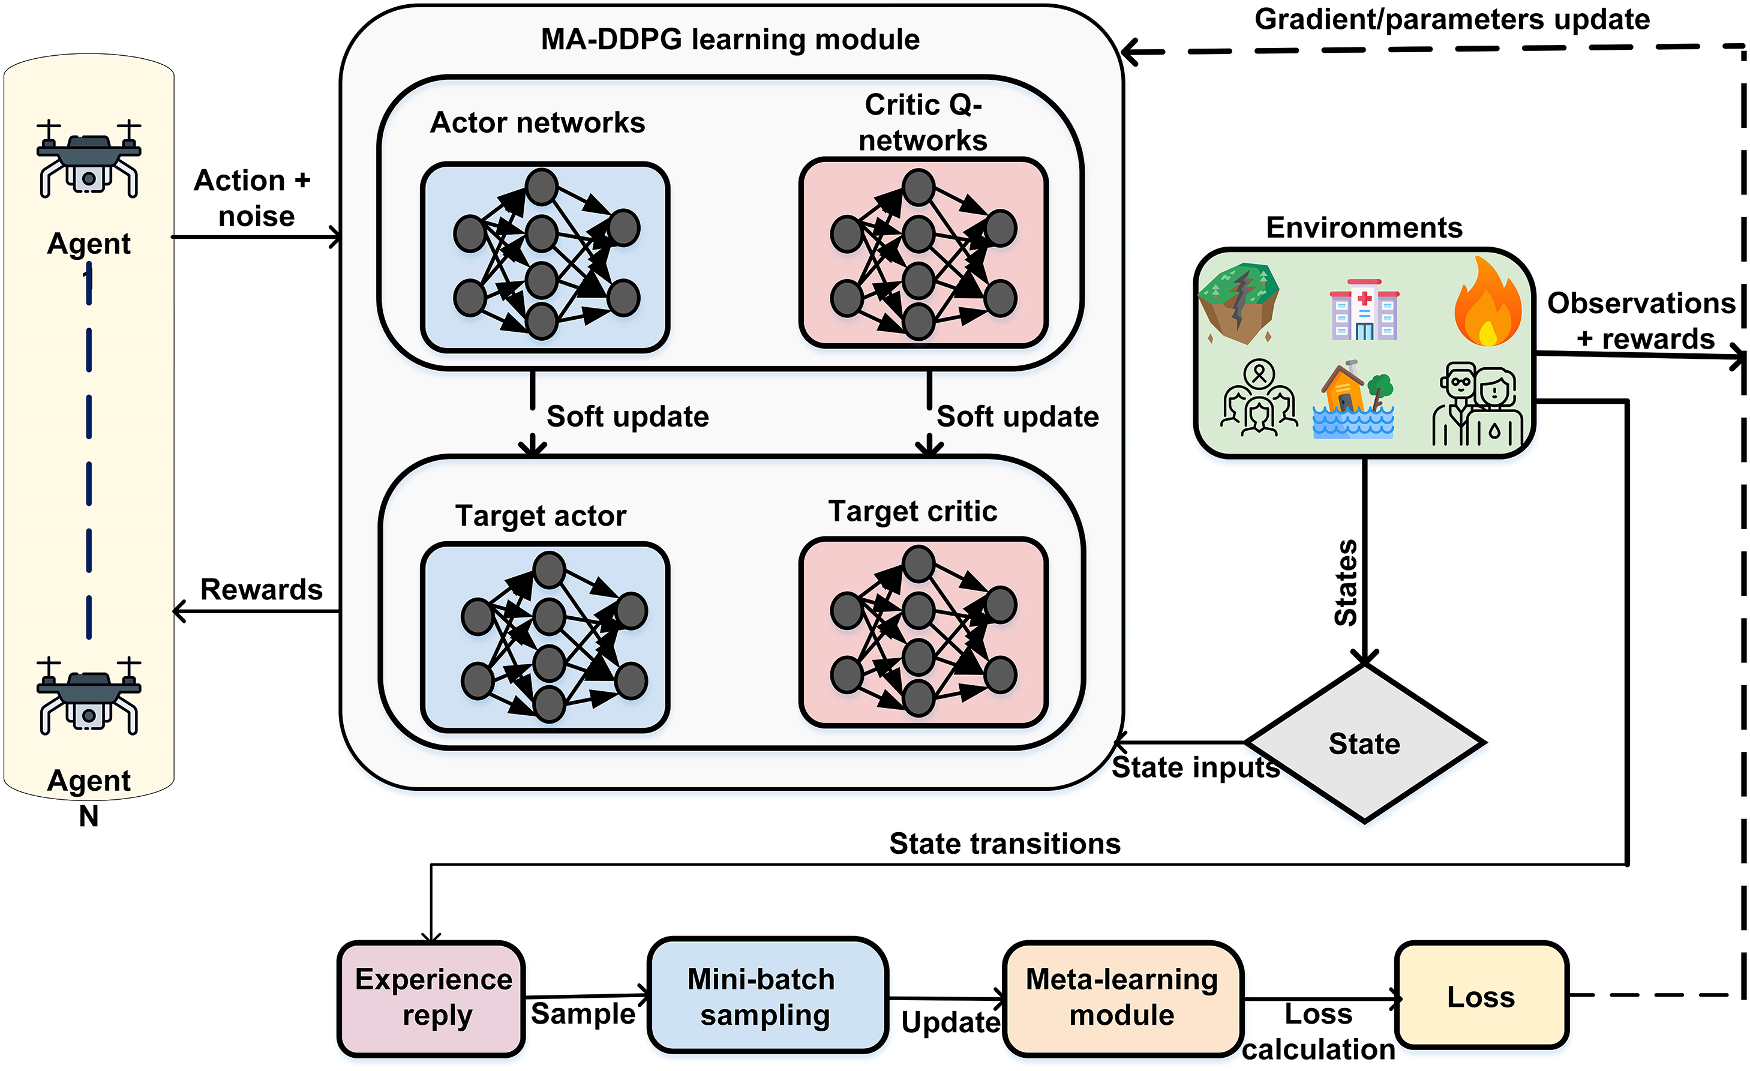
\includegraphics[width=0.90\textwidth]{assets/saras_pipeline_architecture.png}
\caption{Comprehensive multi-tier pipeline architecture of the SARAS disaster response framework}
\label{fig:pipeline}
\end{figure}

\section{Dataset Description}

The edge perception model was trained and evaluated using the benchmark \textbf{VisDrone} aerial dataset \cite{16}, augmented with low-altitude disaster simulation captures:
\begin{itemize}
    \item \textbf{Source and Scale:} The VisDrone dataset was captured by the AISKYEYE team across diverse geographical regions, flying multi-rotor camera platforms at altitudes ranging from 5 meters to 80 meters above ground level. It consists of 10,209 static image captures (6,471 training images, 548 validation images, and 3,190 testing images).
    \item \textbf{Class Distribution:} The dataset encompasses 10 distinct object categories. To tailor the detector specifically for search and rescue operations, annotations were filtered and consolidated into two core target categories: \textit{Pedestrian/Person} (representing standing, walking, prone, or trapped human victims) and \textit{Vehicle} (serving as negative contextual distractors or rescue vehicular ground references).
    \item \textbf{Scale and Occlusion Challenges:} The dataset presents extreme scale variation: over 62\% of the target annotations occupy bounding box areas smaller than $32 \times 32$ pixels, closely emulating high-altitude post-disaster search scenarios. Furthermore, severe object occlusions (ranging from 10\% to 70\% overlap by foliage, rubble, or dust) provide a rigorous testbed for model robustness.
\end{itemize}

\section{Data Preprocessing and Augmentation}

To prepare the aerial imagery for efficient embedded training and inference, a five-stage preprocessing pipeline was implemented:
\begin{enumerate}
    \item \textbf{Annotation Sanitization and Filtering:} Corrupted bounding boxes containing negative coordinates, zero-area dimensions, or out-of-boundary artifacts were programmatically pruned. Target class labels were mapped to standard YOLO format: $\langle\text{class\_id}, x_{\text{center}}, y_{\text{center}}, w, h\rangle$, normalized within $[0.0, 1.0]$.
    \item \textbf{Adaptive Letterbox Resizing:} Training raw drone imagery directly at native 4K or 1080p resolutions causes prohibitive computational overhead. Images were adaptively resized to an optimal input resolution of $640 \times 640 \times 3$ pixels using letterbox padding. The aspect ratio was preserved by scaling the longest dimension and padding remaining borders with neutral gray pixels ($RGB = [114, 114, 114]$), avoiding aspect ratio distortion of prone human silhouettes.
    \item \textbf{Pixel Normalization:} Pixel intensities were normalized from the standard integer range $[0, 255]$ to floating-point values in $[0.0, 1.0]$ via affine scaling:
    \begin{equation}
        I_{\text{norm}}(x, y) = \frac{I(x, y)}{255.0}
    \end{equation}
    \item \textbf{Class Imbalance Mitigation via Dynamic Loss Weighting:} Due to the severe disproportion between small person targets and large background landscapes, class weighting factors were incorporated into the focal loss objectives, inversely proportional to class frequencies across the training corpus.
    \item \textbf{Data Augmentation Strategy:} To prevent overfitting on specific lighting and weather domains, training batches underwent stochastic data augmentations:
    \begin{itemize}
        \item \textit{Mosaic Augmentation:} Combines 4 random training images into a single synthetic training frame, forcing the network to localize targets across four distinct scales and border contexts.
        \item \textit{MixUp Augmentation:} Linearly blends two images and their target labels with a mixing coefficient $\alpha = 0.2$.
        \item \textit{Affine and Photometric Perturbations:} Random horizontal flips ($p=0.5$), rotation within $\pm 10^\circ$, perspective jitter ($\pm 0.001$), and HSV color gamut adjustments (hue: $\pm 0.015$, saturation: $\pm 0.7$, value: $\pm 0.4$).
    \end{itemize}
\end{enumerate}

\section{Feature Extraction and Representation}

The perception backbone leverages a deep Cross-Stage Partial Darknet (CSPDarknet) architecture engineered to balance semantic representation capacity against computational footprint. 

The network extracts features at multiple spatial resolutions, constructing a hierarchical feature pyramid:
\begin{itemize}
    \item Low-level spatial features ($P_3$, stride 8, resolution $80 \times 80$) capture fine-grained texture and localized edge gradients essential for resolving tiny, distant human victims.
    \item Intermediate semantic features ($P_4$, stride 16, resolution $40 \times 40$) integrate medium-scale structural details.
    \item High-level abstract features ($P_5$, stride 32, resolution $20 \times 20$) possess large receptive fields, capturing contextual environmental markers (such as roadway boundaries or riverbank margins).
\end{itemize}
The extracted multi-scale representations are routed through a Path Aggregation Network (PANet) neck, which implements bidirectional top-down and bottom-up feature fusion pathways. This architecture guarantees that rich semantic context flows downward while high-frequency localization cues propagate upward, maximizing detection sensitivity for victims partially occluded by natural or structural debris.

\section{Proposed Model Architecture}

To ensure high-speed onboard execution on resource-constrained embedded companion processors (e.g., Raspberry Pi 4 with 4 GB LPDDR4 RAM), the detection framework was designed around an anchor-free, decoupled head architecture:
\begin{itemize}
    \item \textbf{Anchor-Free Detection Paradigm:} Traditional anchor-based detectors (e.g., YOLOv4, Faster R-CNN) require manual tuning of anchor box aspect ratios, which severely degrades when aerial altitude or camera tilt angles fluctuate. The proposed anchor-free head directly predicts the distance from target grid cells to the four boundaries of the ground truth box, substantially reducing hyperparameter sensitivity and post-processing latency.
    \item \textbf{Decoupled Classification and Regression Heads:} For each feature pyramid scale ($P_3, P_4, P_5$), feature maps branch into two independent sub-networks: a classification head computing class probabilities, and a regression head predicting bounding box offsets. Decoupling resolves the inherent objective conflict between category identification and spatial boundary localization.
    \item \textbf{Parameter Footprint:} The engineered nano model comprises approximately 3.2 million trainable parameters and requires 8.7 Giga-Floating Point Operations (GFLOPs) per forward pass at $640 \times 640$ resolution. When converted to an INT8 quantized representation, the model occupies less than 6.4 MB of memory storage, enabling instant cache residency on ARM processors.
\end{itemize}

\section{Loss Function and Optimization}

The network is optimized using a composite multi-task objective function that jointly penalizes spatial localization errors, bounding box distribution uncertainty, and classification errors:
\begin{equation}
    \mathcal{L}_{\text{total}} = \lambda_{\text{box}} \mathcal{L}_{\text{CIoU}} + \lambda_{\text{dfl}} \mathcal{L}_{\text{DFL}} + \lambda_{\text{cls}} \mathcal{L}_{\text{BCE}}
\end{equation}
where $\lambda_{\text{box}} = 7.5$, $\lambda_{\text{dfl}} = 1.5$, and $\lambda_{\text{cls}} = 0.5$ are balancing hyperparameters empirically validated on aerial benchmarks.

\subsection{Complete Intersection over Union ($\mathcal{L}_{\text{CIoU}}$) Loss}
Bounding box regression is penalized using the Complete IoU metric, which accounts for overlap area, centroid distance, and aspect ratio consistency between predicted box $B$ and ground truth box $B^{gt}$:
\begin{equation}
    \mathcal{L}_{\text{CIoU}} = 1 - \text{IoU} + \frac{\rho^2(b, b^{gt})}{c^2} + \alpha v
\end{equation}
where $\text{IoU} = \frac{|B \cap B^{gt}|}{|B \cup B^{gt}|}$, $\rho(b, b^{gt})$ denotes the Euclidean distance between central coordinates, and $c$ is the diagonal length of the smallest enclosing box covering both $B$ and $B^{gt}$. The parameter $v$ measures aspect ratio disparity:
\begin{equation}
    v = \frac{4}{\pi^2} \left( \arctan\frac{w^{gt}}{h^{gt}} - \arctan\frac{w}{h} \right)^2
\end{equation}
and $\alpha$ is a dynamic balancing coefficient defined as:
\begin{equation}
    \alpha = \frac{v}{(1 - \text{IoU}) + v}
\end{equation}

\subsection{Distribution Focal Loss ($\mathcal{L}_{\text{DFL}}$)}
To address ambiguous object boundaries caused by partial occlusion and sensor motion blur, the regression head models boundary offsets as continuous probability distributions over a discrete set of bins $\{y_0, y_1, \dots, y_n\}$:
\begin{equation}
    \mathcal{L}_{\text{DFL}}(S_i, S_{i+1}) = - \left( (y_{i+1} - y) \log(S_i) + (y - y_i) \log(S_{i+1}) \right)
\end{equation}
where $y_i \le y \le y_{i+1}$ represents the ground truth coordinate, and $S_i$ represents the softmax output of bin $i$.

\subsection{Classification Loss ($\mathcal{L}_{\text{BCE}}$)}
Target category classification is trained via Binary Cross-Entropy (BCE) with sigmoid activation across all detection heads:
\begin{equation}
    \mathcal{L}_{\text{BCE}} = - \frac{1}{N} \sum_{i=1}^N \left[ y_i \log(\hat{p}_i) + (1 - y_i) \log(1 - \hat{p}_i) \right]
\end{equation}
where $y_i \in \{0, 1\}$ denotes the binary ground truth class label and $\hat{p}_i \in [0, 1]$ represents the predicted category confidence score.

\subsection{Optimization and Learning Rate Scheduling}
The optimization procedure employs the AdamW (Adaptive Moment Estimation with Decoupled Weight Decay) algorithm with momentum parameters $\beta_1 = 0.937$ and $\beta_2 = 0.999$, paired with a weight decay factor $\omega = 0.0005$. Training executes under a Cosine Annealing learning rate schedule initialized at $\eta_0 = 0.01$ and decaying to $\eta_{\text{min}} = 0.0001$:
\begin{equation}
    \eta_t = \eta_{\text{min}} + \frac{1}{2}(\eta_0 - \eta_{\text{min}})\left(1 + \cos\left(\frac{t}{T_{\text{max}}}\pi\right)\right)
\end{equation}
where $t$ represents the current training epoch and $T_{\text{max}}$ denotes total training duration. A 3-epoch linear warm-up phase prevents gradient explosion during early weight updates.

\section{Training Strategy}

The network was trained using a disciplined multi-stage transfer learning protocol:
\begin{itemize}
    \item \textbf{Transfer Learning from Pre-Trained Weights:} Model weights were initialized from the MS COCO (Common Objects in Context) pre-trained checkpoint. Pre-training on 80 generalized object classes provides rich low-level spatial filtering primitives, accelerating convergence on aerial domains.
    \item \textbf{Two-Stage Fine-Tuning:} During the first 10 epochs, backbone convolution layers were frozen to allow the randomly initialized detection heads to stabilize their gradient trajectories without corrupting foundational feature representations. In the subsequent 90 epochs, all layers were unfrozen for end-to-end backpropagation.
    \item \textbf{Early Stopping and Regularization:} Model performance was validated at the conclusion of every epoch on the VisDrone validation split. An early stopping patience threshold of 15 epochs was enforced against validation mAP, preventing overfitting on training artifacts.
    \item \textbf{Post-Training Quantization (PTQ):} Following FP32 convergence, the model weights and activations were converted to 8-bit signed integer (INT8) representations using symmetric min-max calibration over 500 representative disaster images, reducing computational memory bandwidth without retraining.
\end{itemize}

\section{Evaluation Metrics}

Model perception and swarm coordination are assessed across rigorous, mathematically defined benchmark metrics:

\subsection{Perception Evaluation Metrics}
\begin{itemize}
    \item \textbf{Precision ($P$):} The proportion of detected candidate victims that are genuine human subjects:
    \begin{equation}
        P = \frac{TP}{TP + FP}
    \end{equation}
    \item \textbf{Recall ($R$):} The proportion of actual ground truth victims successfully localized by the vision pipeline:
    \begin{equation}
        R = \frac{TP}{TP + FN}
    \end{equation}
    where $TP$, $FP$, and $FN$ represent true positive, false positive, and false negative counts under an IoU threshold of 0.5.
    \item \textbf{F1-Score:} The harmonic mean of precision and recall:
    \begin{equation}
        F_1 = 2 \times \frac{P \times R}{P + R}
    \end{equation}
    \item \textbf{Mean Average Precision ($\text{mAP}$):} Computed as the mean area under the Precision-Recall curve across all evaluated classes:
    \begin{equation}
        \text{AP} = \int_{0}^{1} P(R) \, dR, \quad \text{mAP} = \frac{1}{C}\sum_{k=1}^C \text{AP}_k
    \end{equation}
    Metrics are reported at standard $\text{mAP@0.5}$ and rigorous $\text{mAP@0.5:0.95}$ (averaged over 10 IoU thresholds from 0.50 to 0.95 with steps of 0.05).
    \item \textbf{Inference Latency and Throughput:} Measured in milliseconds per frame ($T_{\text{infer}}$) and Frames Per Second ($\text{FPS} = 1000 / T_{\text{infer}}$) on target embedded hardware.
\end{itemize}

\subsection{Swarm Coordination Evaluation Metrics}
\begin{itemize}
    \item \textbf{Area Coverage Efficiency ($\eta_{\text{cov}}$):} The ratio of unique surveyed area $A_{\text{unique}}$ to total cumulative flight swept area $A_{\text{total}}$:
    \begin{equation}
        \eta_{\text{cov}} = \frac{A_{\text{unique}}}{A_{\text{total}}} \times 100\%
    \end{equation}
    Higher efficiency indicates minimal trajectory overlap between peer drones.
    \item \textbf{Fault Reallocation Latency ($T_{\text{realloc}}$):} The elapsed time from the physical failure of an agent to the successful consensus-based reassignment and trajectory resumption by a surviving peer drone.
\end{itemize}
